%!TEX program = lualatex
% Arquivo: figuras/fluxo_descomissionamento.tex
\documentclass[border=8pt]{standalone}

% ===== Fonte (LuaLaTeX) =====
\usepackage{fontspec}
\setmainfont{Latin Modern Roman}

% ===== Cores / TikZ =====
\usepackage[dvipsnames]{xcolor}
\usepackage{tikz}
\usetikzlibrary{shapes.geometric, arrows.meta, positioning}

% ===== Estilos =====
\tikzset{
  process/.style = {
    rectangle,
    rounded corners,
    minimum width=6.0cm,
    minimum height=1.05cm,
    text centered,
    text width=5.7cm,
    draw=blue!70!black,
    fill=blue!5,
    line width=0.9pt
  },
  process_final/.style = {
    process,
    fill=green!6,
    draw=green!45!black
  },
  arrow/.style = {
    thick,
    ->,
    >=Stealth,
    line width=1.1pt,
    draw=gray!80
  }
}

\begin{document}
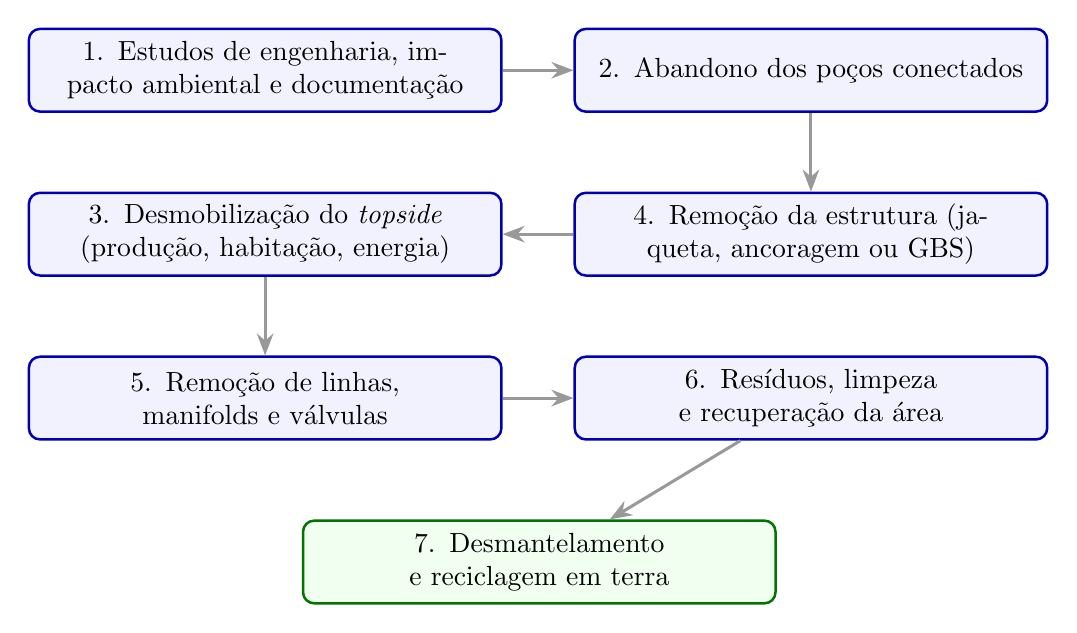
\begin{tikzpicture}[
  node distance=1.0cm and 0.9cm % (vertical) and (horizontal)
]

% ===== Linha 1 (esq -> dir) =====
\node (s1) [process] {1. Estudos de engenharia, impacto ambiental e documentação};
\node (s2) [process, right=of s1] {2. Abandono dos poços conectados};

% ===== Linha 2 (dir -> esq) =====
\node (s4) [process, below=of s2] {4. Remoção da estrutura (jaqueta, ancoragem ou GBS)};
\node (s3) [process, left=of s4] {3. Desmobilização do \textit{topside} (produção, habitação, energia)};

% ===== Linha 3 (esq -> dir) =====
\node (s5) [process, below=of s3] {5. Remoção de linhas, manifolds e válvulas};
\node (s6) [process, right=of s5] {6. Resíduos, limpeza e recuperação da área};

% ===== Linha 4 (final centralizado) =====
\node (s7) [process_final, below=of s6, xshift=-3.45cm] {7. Desmantelamento e reciclagem em terra};

% ===== Setas (fluxo serpente) =====
\draw [arrow] (s1) -- (s2);

\draw [arrow] (s2) -- (s4);        % desce (fim da linha 1 -> topo da linha 2)
\draw [arrow] (s4) -- (s3);        % volta (dir -> esq)

\draw [arrow] (s3) -- (s5);        % desce (fim da linha 2 -> início da linha 3)
\draw [arrow] (s5) -- (s6);        % esq -> dir

\draw [arrow] (s6) -- (s7);        % desce para o final

\end{tikzpicture}
\end{document}
